\documentclass{article}
\usepackage{tikz,amsmath,siunitx}
\usepackage{pgfplots}
\usepackage{listings}
\usetikzlibrary{arrows,snakes,backgrounds,patterns,matrix,shapes,fit,calc,shadows,plotmarks}
%\usepackage[graphics,tightpage,active]{preview}
%\PreviewEnvironment{tikzpicture}
%\PreviewEnvironment{equation}
%\PreviewEnvironment{equation*}
\title{CS540 Practice Assignment 3}
\author{Dustin Ingram}
\newlength{\imagewidth}
\newlength{\imagescale}
\pagestyle{empty}
\thispagestyle{empty}
\lstset{breaklines=true}
\begin{document}
\maketitle
\newpage
\pgfplotsset{width=10cm,compat=1.4}
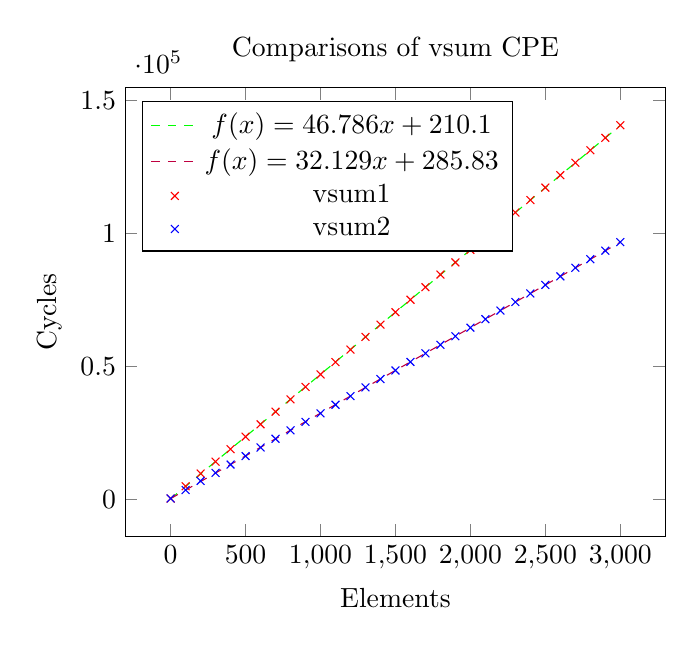
\begin{tikzpicture}
\begin{axis}[
xlabel=Elements,
ylabel=Cycles,
legend pos=north west,
title=Comparisons of vsum CPE] 
\legend{$f(x) = 46.786x + 210.1$, $f(x) = 32.129x + 285.83$, vsum1, vsum2}
\addplot[color=green,dashed] coordinates {
(	0	,	210.1	)
(	100	,	4888.7	)
(	200	,	9567.3	)
(	300	,	14245.9	)
(	400	,	18924.5	)
(	500	,	23603.1	)
(	600	,	28281.7	)
(	700	,	32960.3	)
(	800	,	37638.9	)
(	900	,	42317.5	)
(	1000	,	46996.1	)
(	1100	,	51674.7	)
(	1200	,	56353.3	)
(	1300	,	61031.9	)
(	1400	,	65710.5	)
(	1500	,	70389.1	)
(	1600	,	75067.7	)
(	1700	,	79746.3	)
(	1800	,	84424.9	)
(	1900	,	89103.5	)
(	2000	,	93782.1	)
(	2100	,	98460.7	)
(	2200	,	103139.3	)
(	2300	,	107817.9	)
(	2400	,	112496.5	)
(	2500	,	117175.1	)
(	2600	,	121853.7	)
(	2700	,	126532.3	)
(	2800	,	131210.9	)
(	2900	,	135889.5	)
(	3000	,	140568.1	)
};
\addplot[color=purple,dashed] coordinates {
    (   0   ,   285.83  )
    (   100 ,   3498.73 )
    (   200 ,   6711.63 )
    (   300 ,   9924.53 )
    (   400 ,   13137.43    )
    (   500 ,   16350.33    )
    (   600 ,   19563.23    )
    (   700 ,   22776.13    )
    (   800 ,   25989.03    )
    (   900 ,   29201.93    )
    (   1000    ,   32414.83    )
    (   1100    ,   35627.73    )
    (   1200    ,   38840.63    )
    (   1300    ,   42053.53    )
    (   1400    ,   45266.43    )
    (   1500    ,   48479.33    )
    (   1600    ,   51692.23    )
    (   1700    ,   54905.13    )
    (   1800    ,   58118.03    )
    (   1900    ,   61330.93    )
    (   2000    ,   64543.83    )
    (   2100    ,   67756.73    )
    (   2200    ,   70969.63    )
    (   2300    ,   74182.53    )
    (   2400    ,   77395.43    )
    (   2500    ,   80608.33    )
    (   2600    ,   83821.23    )
    (   2700    ,   87034.13    )
    (   2800    ,   90247.03    )
    (   2900    ,   93459.93    )
    (   3000    ,   96672.83    )
};

\addplot[color=red,mark=x, only marks] coordinates {
(   0   ,   309 )
(   100 ,   4932    )
(   200 ,   9735    )
(   300 ,   14196   )
(   400 ,   18890   )
(   500 ,   23558   )
(   600 ,   28226   )
(   700 ,   32964   )
(   800 ,   37590   )
(   900 ,   42276   )
(   1000    ,   46954   )
(   1100    ,   51620   )
(   1200    ,   56312   )
(   1300    ,   61075   )
(   1400    ,   65682   )
(   1500    ,   70368   )
(   1600    ,   75048   )
(   1700    ,   79764   )
(   1800    ,   84499   )
(   1900    ,   89079   )
(   2000    ,   93768   )
(   2100    ,   98439   )
(   2200    ,   103110  )
(   2300    ,   107813  )
(   2400    ,   112500  )
(   2500    ,   117190  )
(   2600    ,   121860  )
(   2700    ,   126532  )
(   2800    ,   131226  )
(   2900    ,   135893  )
(   3000    ,   140634  )
  };
\addplot[color=blue,mark=x, only marks] coordinates {
(   0   ,   348 )
(   100 ,   3516    )
(   200 ,   6942    )
(   300 ,   9963    )
(   400 ,   13098   )
(   500 ,   16287   )
(   600 ,   19500   )
(   700 ,   22791   )
(   800 ,   25951   )
(   900 ,   29139   )
(   1000    ,   32352   )
(   1100    ,   35580   )
(   1200    ,   38799   )
(   1300    ,   42086   )
(   1400    ,   45240   )
(   1500    ,   48453   )
(   1600    ,   51666   )
(   1700    ,   54878   )
(   1800    ,   58092   )
(   1900    ,   61320   )
(   2000    ,   64540   )
(   2100    ,   67752   )
(   2200    ,   70966   )
(   2300    ,   74192   )
(   2400    ,   77405   )
(   2500    ,   80620   )
(   2600    ,   83832   )
(   2700    ,   87060   )
(   2800    ,   90280   )
(   2900    ,   93492   )
(   3000    ,   96706   )
};
\end{axis}
\end{tikzpicture}

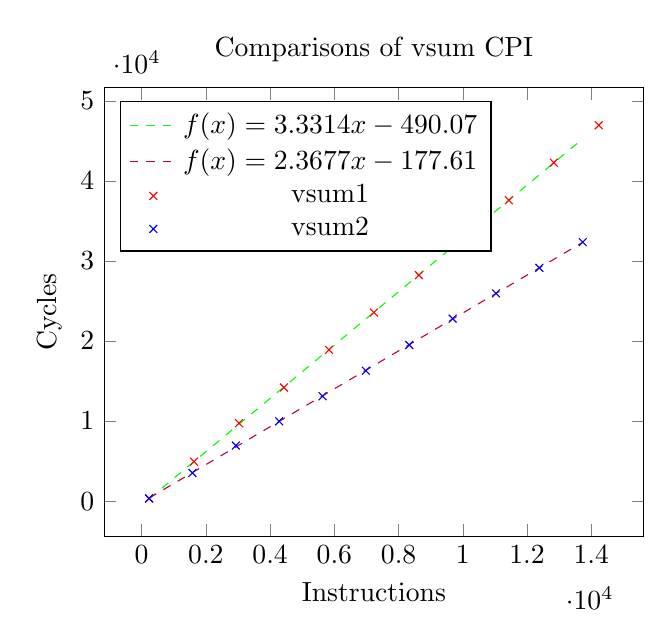
\begin{tikzpicture}
\begin{axis}[
xlabel=Instructions,
ylabel=Cycles,
legend pos=north west,
title=Comparisons of vsum CPI] 
\legend{$f(x) = 3.3314x -490.07$, $f(x) = 2.3677x - 177.61$, vsum1, vsum2}
\addplot[color=green,dashed] coordinates {
(   232 ,   282.8148    )
(   1582    ,   4780.2048   )
(   2932    ,   9277.5948   )
(   4282    ,   13774.9848  )
(   5632    ,   18272.3748  )
(   6982    ,   22769.7648  )
(   8332    ,   27267.1548  )
(   9682    ,   31764.5448  )
(   11032   ,   36261.9348  )
(   12382   ,   40759.3248  )
(   13732   ,   45256.7148  )

};

\addplot[color=purple,dashed] coordinates {
(   232 ,   371.6964    )
(   1582    ,   3568.0914   )
(   2932    ,   6764.4864   )
(   4282    ,   9960.8814   )
(   5632    ,   13157.2764  )
(   6982    ,   16353.6714  )
(   8332    ,   19550.0664  )
(   9682    ,   22746.4614  )
(   11032   ,   25942.8564  )
(   12382   ,   29139.2514  )
(   13732   ,   32335.6464  )
};

\addplot[color=red,mark=x, only marks] coordinates {
(   232 ,   309 )
(   1632    ,   4932    )
(   3032    ,   9735    )
(   4432    ,   14196   )
(   5832    ,   18890   )
(   7232    ,   23558   )
(   8632    ,   28226   )
(   10032   ,   32964   )
(   11432   ,   37590   )
(   12832   ,   42276   )
(   14232   ,   46954   )
};

\addplot[color=blue,mark=x, only marks] coordinates {
(   232 ,   348 )
(   1582    ,   3516    )
(   2932    ,   6942    )
(   4282    ,   9963    )
(   5632    ,   13098   )
(   6982    ,   16287   )
(   8332    ,   19500   )
(   9682    ,   22791   )
(   11032   ,   25951   )
(   12382   ,   29139   )
(   13732   ,   32352   )
};

\end{axis}
\end{tikzpicture}
\newpage
\begin{lstlisting}
$ uname -a
Linux tux64-11.cs.drexel.edu 2.6.35-28-generic #50-Ubuntu SMP Fri Mar 18 18:42:20 UTC 2011 x86_64 GNU/Linux
\end{lstlisting}

\begin{lstlisting}
$ gcc --version
gcc (Ubuntu/Linaro 4.4.4-14ubuntu5) 4.4.5
\end{lstlisting}

\begin{lstlisting}
$ cat /proc/cpuinfo
processor   : 31
vendor_id   : AuthenticAMD
cpu family  : 16
model       : 9
model name  : AMD Opteron(tm) Processor 6136
stepping    : 1
cpu MHz     : 800.000
cache size  : 512 KB
physical id : 3
siblings    : 8
core id     : 3
cpu cores   : 8
apicid      : 71
initial apicid  : 55
fpu     : yes
fpu_exception   : yes
cpuid level : 5
wp      : yes
flags       : fpu vme de pse tsc msr pae mce cx8 apic sep mtrr pge mca cmov pat pse36 clflush mmx fxsr sse sse2 ht syscall nx mmxext fxsr_opt pdpe1gb rdtscp lm 3dnowext 3dnow constant_tsc rep_good nonstop_tsc extd_apicid amd_dcm pni monitor cx16 popcnt lahf_lm cmp_legacy svm extapic cr8_legacy abm sse4a misalignsse 3dnowprefetch osvw ibs skinit wdt nodeid_msr npt lbrv svm_lock nrip_save
bogomips    : 4800.16
TLB size    : 1024 4K pages
clflush size    : 64
cache_alignment : 64
address sizes   : 48 bits physical, 48 bits virtual
power management: ts ttp tm stc 100mhzsteps hwpstate
\end{lstlisting}


\end{document}
